\chapter{Ma collaboration au projet}\label{collab}
\putminitoc
Après avoir défini les besoins de notre outil et son fonctionnement général, nous allons maintenant voir en détail de quelle manière j'ai contribué à ce projet. Le développement s'est effectué en deux grandes étapes. D'une part, la finalisation de la première version via la production de rapports détaillés, et ce jusqu'en janvier. Suivi par des améliorations afin que l'outil puisse être utilisé par le plus grand nombre, notamment par les équipes des projets Renault. 

Dans ce chapitre, nous allons voir quatre des contributions les plus importantes que j'ai effectué durant cette année d'alternance.

\section{La difficulté de productions de rapports}\index{Rapport}
La production de rapport est le cœur de notre plateforme. Ces rapports doivent être fiable, afin d'éviter de faire perdre du temps à l'utilisateur en cas de faux rouge, et ne pas manquer de bogue, en cas de faux vert. 

Au début du développement de l'outil, une solution avait été mise en place, cependant celle-ci avait été effectuée de façon naïve et ne pouvait fonctionner. C'est ainsi qu'en août, nous avons commencé la conception d'un autre algorithme de production de verdicts, basé sur les récurrence de calculs et le concept d'entrées et de sorties de calculs. 

\subsection{Les calculs du logiciel}\index{Récurrence}\index{Tâche}
	Un logiciel embarqué temps réel effectue différents tâches de calculs à des récurrences fixes. C'est-à-dire que le système doit être déterministe et avoir des tâches qui s'exécutent après un temps donné, moyennant une petite marge d'erreur. Dans les logiciels que nous testons, ces tâches peuvent être exécutées toutes les dix millisecondes par exemple. 
	
	Une tâche de calcul prends des donnés en entrée, et écrit un résultat dans une ou plusieurs variables de sortie. Dans le cadre de l'intégration du plugin, un certain nombre de tâche ont pour but la connexion de ce plugin. Ainsi, elles vont prendre les des données du plugin en entrée, et écrire le résultat dans une variable de chez Continental. 

\subsection{Le problème de l'existant}
\begin{figure}[H]
\centering
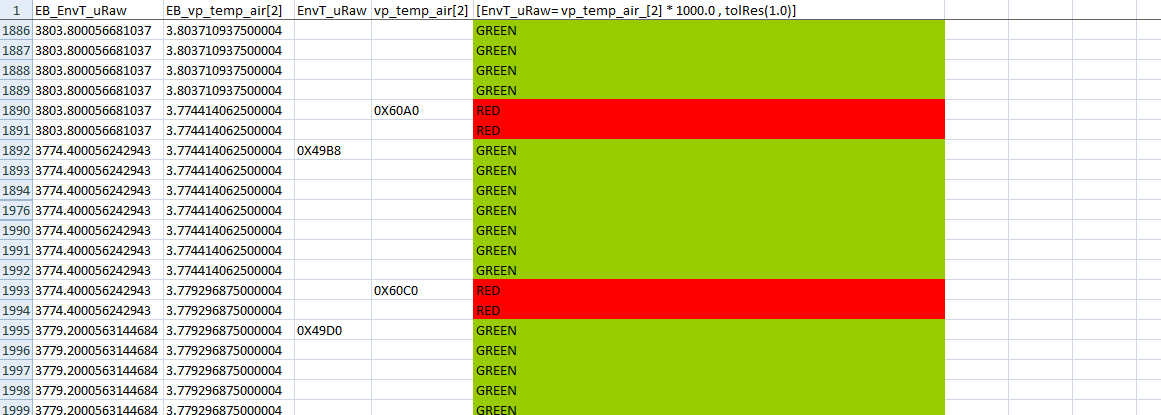
\includegraphics[width=1\linewidth]{contents/images/badReport}
\caption{Exemple d'un rapport incorrect}
\label{fig:badReport}
\end{figure}
\index{Échantillonage}
En début du projet, il avait été décidé que nous allions évaluer une trace à l'ensemble des instants, comme le montre la figure \ref{fig:badReport}. Malheureusement, comme nous pouvons le voir, cette solution ne peut fonctionner. En effet, le \textit{debugger} échantillonne beaucoup plus rapidement que la récurrence des tâches de calculs. Ainsi, nous voyons des changements de valeurs d'états intermédiaires.

Or, l'\textit{expected behavior} qui nous est fourni ne peut être vrai à tout instant de la trace, mais doit être vrai à la fin de notre tâche. Pendant l'exécution d'une tâche, ou avant notre tâche, nous pouvons voir des changements sur des variables d'entrée et être dans un état incohérent : ces états ne nous intéressent pas, et ne doivent pas être pris en comptes, sinon, nous allons dire rouge sur des instants qui ne sont pas significatifs pour l'utilisateur.

Dans la figure \ref{fig:badReport}, nous devons évaluer l'\textit{expected behavior} \texttt{Envt\_uRaw=vp\_temp\_air[2] * 1000}, or nous l'évaluons à tous les instants. Nous prononçons rouge à la ligne 1890, car \texttt{vp\_temp\_air[2]} a changé\ldots Mais \texttt{EnvT\_uRaw} n'a pas eu le temps de s'adapter : il est nécessaire d'attendre sa mise à jour avant de prononcer un réel bogue.

\subsection{Produire un verdict fiable}\index{Verdict}
La solution qui a été trouvée est d'utiliser le concept de variables d'entrées et de sorties vu précédemment. Nous savons que la tâche de calcul est terminée lorsque la variable de sortie est rafraichie.  

Ainsi, un verdict est prononcé uniquement aux rafraichissements de la variable de sortie, entre temps, si les variables d'entrées changent, le verdict est interpolé : nous sommes dans un état intermédiaire. Figure \ref{fig:goodReport} montre le rapport du même test que précédemment, avec une prononciation de verdict correcte. 

\begin{figure}[h]
\centering
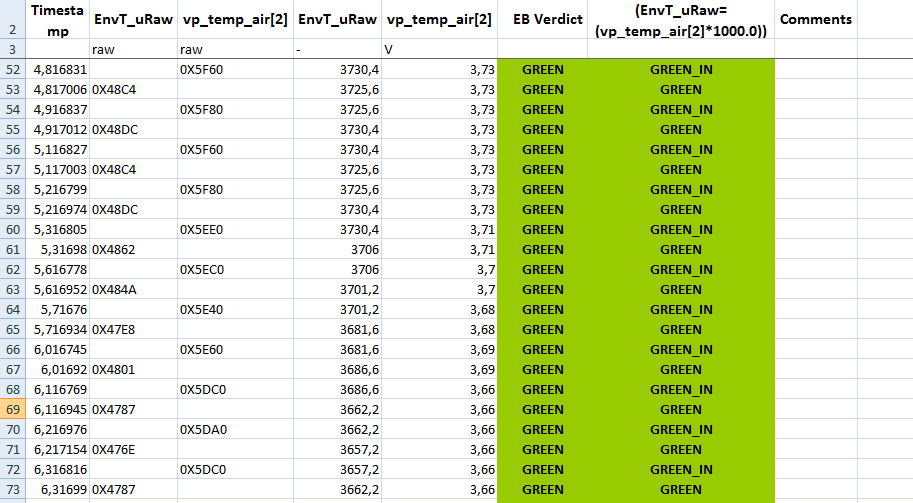
\includegraphics[width=0.9\linewidth]{contents/images/goodReport}
\caption{Exemple d'un rapport correct}
\label{fig:goodReport}
\end{figure}

Comme nous pouvons le voir, l'\textit{expected behavior} est la même, mais cette fois-ci, le verdict est prononcé de la bonne manière. Nous mettons « \texttt{GREEN} » lorsque la variable de sortie, \texttt{EnvT\_uRaw} change de valeur, et dans les autres cas nous interpolons le verdict, en l'occurence \texttt{GREEN}. D'où le \texttt{GREEN\_IN}.
%Nous avons eu du mal à produire des résultats de tests fiables et efficaces : il a fallut adapter notre "analyzer" produisant ces résultats afin qu'il fonctionne dans tous les cas possible, ceci en se servant du concept des récurrences de calcul, et des variables d'entrée et de sortie d'un calcul. Rapide présentation de la sérialisation au format excel


\section{L'arrivée des projets multi-cœurs}\index{Multi-cœur}\index{Panther}
Jusqu'à maintenant, les calculateurs des contrôles moteur fonctionnaient tous en mono-cœur. Ainsi un seul c\oe{}ur effectuait les opérations, et il n'y avait pas de parallélisation. Ce type de calculateur était utilisé pour la première phase des projets Ford, le Panther Phase 1. Or, le projet GreenT avait pour but premier d'être utilisable pour tous les projets Ford, et notamment le panther phase 2. Celui-ci contient beaucoup de variances logicielles ou hardware, ainsi cette base principale est dérivée en plusieurs projets distincts (FPC, FPD, FPE, FPF, \ldots) en fonction des applications. Tous ces projets utilisent des calculateurs multi-cœur, possédant 3 c\oe{}ur distincts. 

Or, GreenT ayant été initialement conçu pour le Panther Phase 1, nous n'avions pas prévu l'utilisation de l'outil pour des projets multi-cœur. Afin de répondre aux besoins de l'équipe, et dans un but de généralisation de notre outil au plus grand nombre, il a été nécessaire d'étudier l'utilisabilité de l'outil dans ce contexte particulier.

\subsection{Analyse d'impacts}\label{analyseimpact}\index{ECU}
Afin de pouvoir mettre en place notre outil sur les projets multi-cœur, il a d'abord fallu énumérer les actions qui sont faites sur l'ECU par notre plateforme, et ensuite vérifier d'éventuelles différences : 
\begin{itemize}
	\item flasher un logiciel,
	\item lire et écrire sur une adresse RAM,
	\item changer la valeur d'une calibration en flash,
	\item démarrer le logiciel (CPU GO),
	\item arrêter le logiciel,
	\item enregistrer une trace.
\end{itemize}


\subsubsection{Le fonctionnement d'un calculateur multi-cœur}\index{ECU}\index{Multi-cœur}
Tout d'abord, afin de pouvoir observer les éventuels modifications à apporter, il faut connaître les spécifications d'un ECU multi-cœur. 
\begin{description}
	\item[Calculs] Le principal problème de notre calculateur, celui-ci possède 3 cœurs distincts qui sont indépendants, ils se démarrent ou s'arrêtent indépendamment. 
	\item[RAM] Chaque c\oe{}ur possède une RAM dite << préférentielle >>, ces différentes adresses RAM auront des accès plus rapide. Cependant, chaque cœur peut accéder à l'ensemble des adresses RAM. Dans le cadre des projets Ford, toutes les variables nécessaires à nos tests sont sur le même c\oe{}ur, le c\oe{}ur 0. 
	\item[Flash] Une seule mémoire flash, ce stockage est indépendant des différents c\oe{}urs. 
\end{description}

Afin de faire fonctionner notre outil, nous allons devoir : 
\begin{itemize}
	\item démarrer ou arrêter l'ensemble des c\oe{}urs en fonction de l'action qui est souhaitée,
	\item lire ou écrire dans les cases RAM depuis le c\oe{}ur 0,
	\item la flash est indépendante de l'architecture de notre calculateur.\\
\end{itemize}

\begin{remarque}\index{Breakpoints}
Actuellement notre outil n'utilise pas le concept de \textit{breakpoints}. Ce type d'utilisation aurait un impact fort sur notre outil, étant donné que pour du multi-cœur, il serait nécessaire de choisir quel c\oe{}ur arrêter, ceux-ci étant indépendant. Si ce besoin se fait sentir, il sera nécessaire de prévoir ce cas d'utilisation.
\end{remarque}

\subsubsection{Le fonctionnement du \textit{debugger} multi-cœur}\index{Device!Debugger}\index{Mono-core}
Le \textit{debugger} Lauterbach multi-cœur est le même que les \textit{debuggers} mono-cœur. La seule différence est la nécessité d'une licence spécifique, actuellement tous les projets possèdent cette licence sur les différents équipements. 

Le debuggage sur projet multi-cœur implique d'avoir une fenêtre du \textit{debugger} par cœur, ainsi nous aurons trois fenêtres, respectivement pour les cœurs 0, 1 et 2. L'outil Trace32 possède une fonctionnalité permettant de « synchroniser » les cœurs, ainsi il est possible de le configurer afin que toute les commandes envoyées sur le cœur 0 soit automatiquement envoyée sur les deux autres cœurs. 

Cela nous permet notamment de pouvoir démarrer ou arrêter les 3 c\oe{}urs au même instant de façon simple. 

\subsection{Les changements de notre outil}
Comme nous avons pu le voir section \ref{analyseimpact}, ce changement majeur pour les projets n'aura que peu d'impact sur notre outil.

Une fois l'analyse d'impact effectuée, il a fallut adapter nos outils pour deux actions : 
\begin{itemize}
	\item le démarrage et l'arrêt du programme,
	\item prendre en compte des temps de réactions de Trace32 différents.
\end{itemize} 

\subsubsection{Le démarrage et l'arrêt du programme}
Comme expliqué précédemment, pour démarrer ou arrêter le programme, il est nécessaire de démarrer ou d'arrêter les trois cœurs simultanément. Pour cela, il a suffit qu'au démarrage de Trace32, notre outil configure celui-ci afin de synchroniser l'appel des commandes des trois cœurs. En effectuant un CPU GO, la commande est envoyé automatiquement aux deux autres cœurs.

\subsubsection{Les temps de réactions}
Le \textit{debugger} possédant trois fenêtres, il a tout de même fallu adapter des temps de réactions qui sont plus longs, notamment pour le démarrage de l'outil, l'arrêt de celui-ci, le flash d'un logiciel, etc… En effet, sans adaptation de ces temps, l'outil renvoyait des exceptions << \textit{timeout} >>.

\subsubsection{Les autres actions}
Nous n'avons eu aucun changement à effectuer pour les autres actions faites par notre outil. En effet, par défaut, toutes nos commandes sont envoyées sur le cœur 0. Or, il est possible de lire ou écrire dans la RAM, et de flasher directement depuis le cœur 0, toutes les variables étant accessibles de n'importe quel cœur. 

\section{Ouverture de l'outil à d'autres projets} \label{gttestplan}\index{GTTestPlan}\index{Renault}\index{TestPlan}
Rapidement après la première version multi-cœur de GreenT, le besoin s'est fait sentir d'utiliser GreenT pour certains tests Renault. Or, il n'était actuellement possible de rédiger des tests que via un fichier Walkthrough, avec les bonnes colonnes et les bonnes variables. 

Il était donc nécessaire de pouvoir rédiger un test de manière simple, indépendamment du \textit{Walkthrough}. Pour gagner du temps de développement, il a été choisi d'utiliser ici également un fichier Excel, ce qui permet d'avoir un parser qui ressemblera beaucoup au parser original. Ce fichier Excel générique que j'ai mis au point est présenté figure \ref{fig:gttestplan}. 


\begin{figure}[h]
\hspace{-40px}
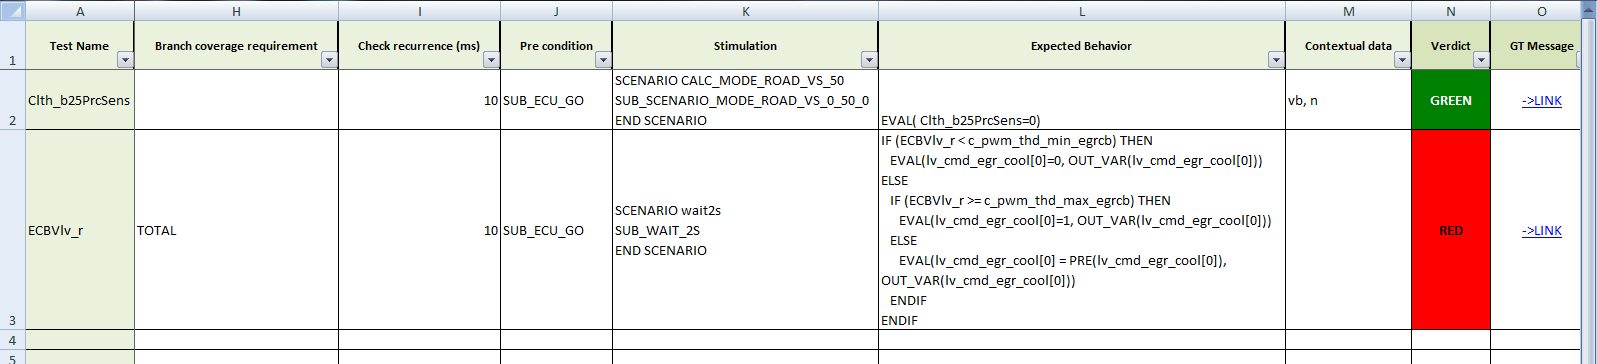
\includegraphics[width=1.15\linewidth]{contents/images/gttestplan}
\caption{Exemple d'un test plan générique}
\label{fig:gttestplan}
\end{figure}

Le fichier de testplan générique contient les informations utiles pour bien effectuer notre test, ainsi il est nécessaire de fournir : 
\begin{itemize}
	\item des informations contextuelles sur le test, tel que le nom, la description, la release concernée, le responsable, l'agrégat,
	\item des informations utiles à l'analyse, tel que le type de test (Calculation, Stub, IO), la récurrence de calcul, la nécessité de couverture des branches (partielle ou totale), et si le test doit être exécuté,
	\item les cellules du test (Précondition, Scenarii de stimulation, \textit{Expected Behavior}, Contextual data),
	\item les cellules remplies après l'exécution, c'est-à-dire le verdict du test, les messages d'erreurs, liens vers le rapport.
\end{itemize}
\index{Excel}
Il suffit à l'utilisateur de remplir ce fichier excel, avec une ligne par test qu'il veut faire, de bien renseigner le type de \textit{testplan} dans le fichier de configuration, et ensuite tout le reste du processus sera le même.

Le développement de cette fonctionnalité a nécessité l'adaptation de l'outil à un autre type de parser que le \textit{Walkthrough}, ce que j'ai mis au point avec un simple héritage, ainsi si un jour nous souhaitons un autre type de parser, tel que du XML, ce sera simple à mettre en place. 

\section{La synchronisation des traces}\label{synchro}\index{Synchronisation}\index{ECU}\index{Plugin}\index{Device}\index{Device!Debugger}\index{Device!HiL}
Dans le cadre des projets Ford, l'équipe avait un besoin unique, celui de comparer des variables de l'ECU entre elle, plus précisément des variables du plugin avec des variables du logiciel Continental.

Afin d'ouvrir l'outil au maximum de projets possibles, un autre besoin est apparu : pouvoir comparer une variable ECU avec un symbole venant du HiL. Ce besoin implique d'avoir deux traces d'exécution différentes, une du \textit{debugger}, et une du HiL. Cette fonctionnalité avait été prévu au tout début du projet, ainsi il est déjà possible d'enregistrer une trace provenant de chacun des deux \textit{devices}, mais par manque de temps, nous avions choisis de mettre la synchronisation de côté.

La plus grande difficulté reste dans la synchronisation des temps du HiL et du \textit{debugger}. En effet, entre le moment où on démarre l'enregistrement côté HiL, et que l'on démarre l'enregistrement côté \textit{debugger}, nous allons avoir un décalage de temps pouvant être conséquent. Afin que GreenT soit capable de prononcer des verdicts entre deux traces différentes, il est nécessaire d'avoir la même base de temps et le même timestamp 0. 

\subsection{Trouver deux signaux comparables}\index{Signal!Analogique}
Pour pouvoir synchroniser deux traces, il est nécessaire d'avoir un signal identique enregistré sur les deux traces. En fonction de la forme de ce signal, il est ensuite possible de synchroniser nos deux traces, ceci à l'aide des fronts montants et fronts descendants par exemple. 

Il est donc nécessaire d'avoir un signal qui soit envoyé par le HiL, vers l'ECU. Ce signal sera ensuite relu côté HiL et lu côté ECU, nous aurons alors deux signaux identiques des deux côtés, moyennant le temps de propagation du matériel, et éventuellement du bruit en fonction de la qualité du signal. 

Afin d'être totalement générique, il est nécessaire de trouver un signal qui soit présent sur l'ensemble des projets, afin de ne pas avoir une solution spécifique à un type de projet (Comme pourrait l'être le signal d'embrayage absent des projets de boite automatique par exemple). Il existe deux types de signaux que nous allons détailler plus bas. 


\subsection{Utiliser un signal analogique : la batterie}\index{Signal!Batterie}
Dans un premier temps, nous avons pensé à un signal qui soit indispensable à l'ensemble des projets, et qui soit facile à contrôler, en ayant aucune incidence sur le calculateur, afin d'éviter des effets de bord. 

Le signal batterie nous a ainsi apparu évident, il nous suffisait d'effectuer un \textit{glitch} sur la batterie avec un certain pattern, en début et en fin de scénario. Ce signal serait enregistré côté HiL et côté ECU.
\begin{figure}[h]
\centering
\vspace{-10px}
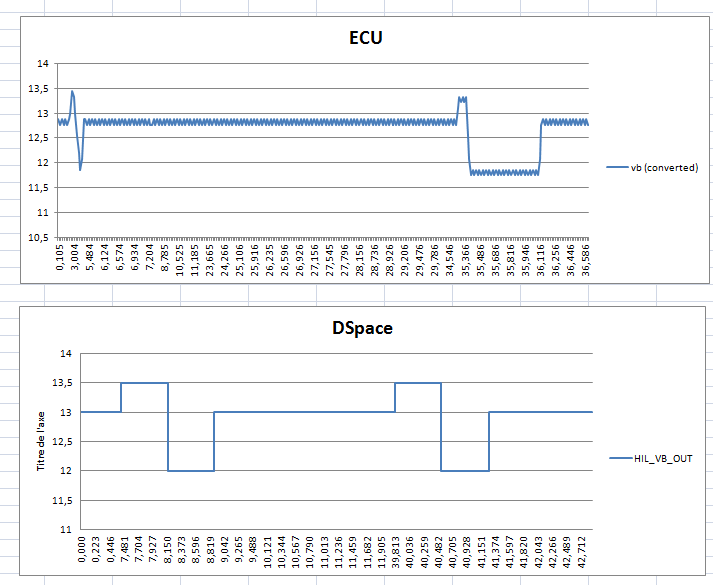
\includegraphics[width=0.61\linewidth]{contents/images/sync1}
\caption{Enregistrement de la batterie côté HiL et côté ECU}
\label{fig:sync-traces-vb}
\end{figure}
\index{Oscilloscope}
Comme nous pouvons le voir, le signal de batterie envoyé par le HiL est particulièrement propre, ce qui est normal étant donné que c'est lui qui le génère. Le principal problème vient dans le transport de ce signal jusqu'à l'ECU. Nous pouvons voir que celui-ci est d'une part particulièrement bruité, et d'autre part qu'il est plus faible qu'au départ. Ces problèmes sont matériel, et proviennent principalement du boitier d'éclatement qui est présent en sorti de HiL, afin de laisser la possibilité à certains utilisateurs de relire différents signaux à l'aide d'un oscilloscope par exemple. 

Au vue de ces traces, il est difficile de pouvoir faire correspondre facilement les signaux, en étant certains de ne pas avoir d'erreurs dues au bruit. 

Il semble donc bien plus simple d'utiliser un signal logique, ceux-ci ne pouvait être bruité. Il est ainsi facile de comparer deux signaux logiques via leurs fronts montant ou descendants. 


\subsection{Utiliser le signal logique : le signal clé}\index{Signal!Logique}\index{Signal!Clé}
Comme vu précédemment, le signal logique est bien plus simple à traiter et limite les erreurs dues au bruit. Il est donc nécessaire de trouver un signal logique qui est disponible sur l'ensemble des projets, et qui n'ait aucun impact sur le code du calculateur. En effet, notre signal permettant la synchronisation ne doit pas << polluer >> notre test, afin d'avoir des pré-conditions correctement établies. 

Nous n'avons pas pu trouver un signal correspondant exactement à ces critères, nous avions pensé à la pédale de frein ou d'embrayage, utilisées à l'arrêt, mais d'une part nous ne pouvons garantir l'absence de stratégies en fonction des projets, et d'autre part une voiture automatique ne possèdera pas d'embrayage. Une autre solution a été trouvée : la clé.

La clé possède un certain nombre de stratégies (effacer des erreurs par exemple), cependant il n'est pas possible d'avoir un test ou la clé n'est pas mis à 1, le calculateur n'étant pas alimenté sans clé, aucune trace ne pourrait être enregistrée. De la même manière, un test doit obligatoirement terminer sur une clef à 0, ainsi tous les tests effectués avec GreenT posséderaient les étapes montrées figure \ref{fig:testKey}. 

\begin{figure}[h]
	\centering
	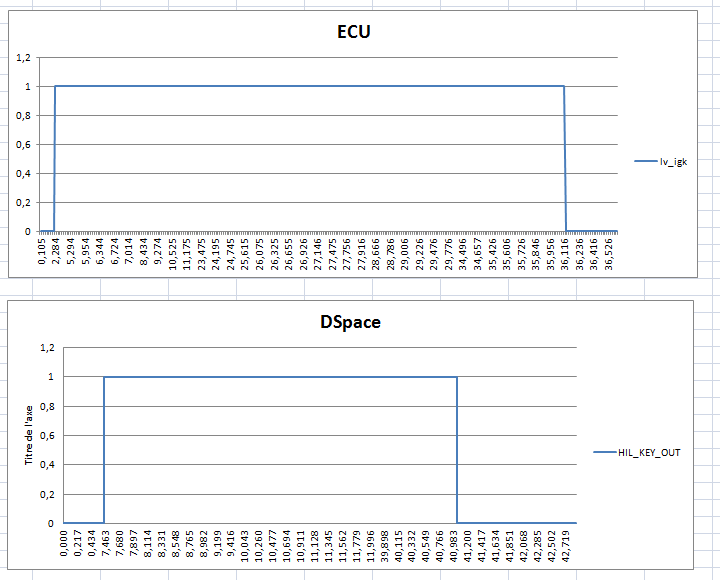
\includegraphics[width=0.61\linewidth]{contents/images/sync2}
	\caption{Enregistrement idéal d'un signal logique, ici la clé}
	\label{fig:testKey}
\end{figure}


Tous les tests possédant ces fronts montants et descendant, il est ainsi possible de synchroniser nos deux traces en enregistrant la clé côté HiL, et côté \textit{debugger}. 

Seulement, comme nous allons le voir, la figure \ref{fig:testKey} montre l'enregistrement idéal. Malheureusement il n'est pas possible d'enregistrer la clé côté ECU de cette manière.

\subsection{Le problème de l'enregistrement de la clé}
Le signal clé semble la solution idéale de synchronisation. Cependant, ce signal est particulier étant donné que c'est sa mise à 1 qui permet d'alimenter le calculateur. Il est donc impossible d'enregistrer un front montant de la clé via le \textit{debugger}, celui-ci fonctionnant avec le port JTag, il est nécessaire que le calculateur soit alimenté. 

\subsubsection{Les traces d'enregistrement}\label{tracesSync}\index{Trace}\index{Lauterbach}\index{Device!Debugger}\index{Device!Powerprobe}
La solution trouvée est d'enregistrer le signal de clé avec un autre équipement fourni par Lauterbach, l'entreprise délivrant le \textit{debugger}. Cet outil est un analyseur logique, appelé \textit{PowerProbe}, qui se branche directement sur le \textit{debugger} via un port série. Il est ainsi possible d'enregistrer le signal clé via un fil allant du HiL jusqu'à l'analyseur logique.

Nous aurons donc trois traces différentes pour la synchronisation : 
\begin{itemize}
	\item la trace venant du HiL, contenant le signal clé,
	\item la trace venant du \textit{PowerProbe}, contenant le signal clé et une pulse de synchronisation,
	\item la trace venant du \textit{debugger}.
\end{itemize}

Le \textit{PowerProbe} étant branché en série sur le \textit{debugger}, il est possible de paramétrer le \textit{debugger} afin d'envoyer une pulse au \textit{PowerProbe} dès que l'ECU est démarré, il suffira ensuite de synchroniser le 0 de la trace \textit{debugger} avec la pulse du \textit{PowerProbe}. Restera à synchroniser la trace du \textit{PowerProbe} avec la trace du HiL en fonction des fronts du signal clé. Figure \ref{fig:tracesigk} est représenté les trois traces qui seront synchronisées. 

\begin{figure}[H]
	\centering
	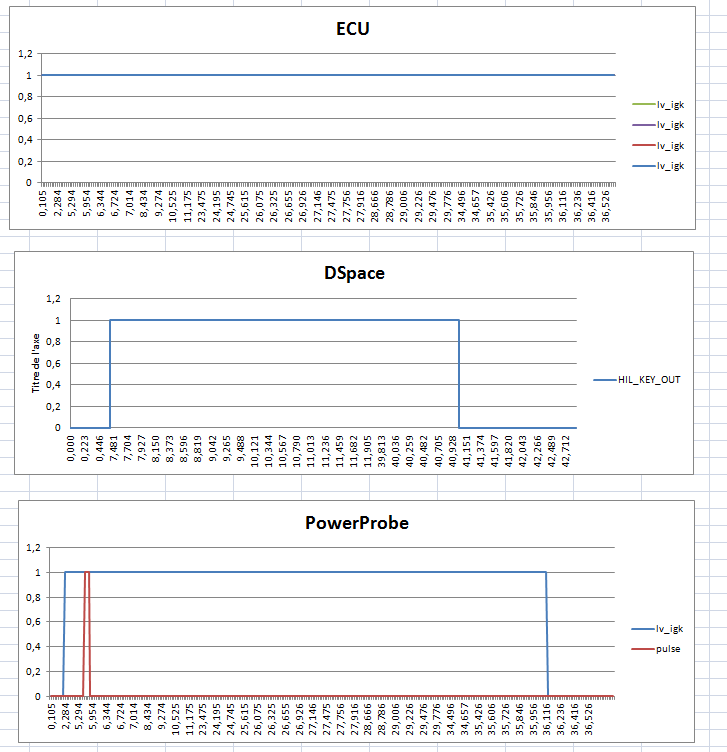
\includegraphics[width=0.61\linewidth]{contents/images/sync3}
	\caption{Enregistrement de la clé sur les trois équipements}
	\label{fig:tracesigk}
\end{figure}

Sur la figure \ref{fig:tracesigk}, nous pouvons observer d'une part l'enregistrement du HiL, qui n'a pas changé, l'enregistrement réel côté ECU qui n'est pas utile, car il n'est capable de ne voir que la clé à 1, et surtout l'enregistrement du \textit{PowerProbe}. On peut voir sur celui-ci la clé, en bleu, ainsi qu'une pulse en rouge correspondant à l'instant ou l'ECU a démarré. 

\subsubsection{La configuration permettant l'enregistrement}
Afin d'avoir les traces comme présentées section  \ref{tracesSync}, il est nécessaire de brancher correctement les équipements sur la table de tests. Cette configuration est légèrement différentes que lorsque nous n'avons pas de synchronisation, celle-ci est détaillé dans la figure \ref{fig:tracesSync}.

\begin{figure}[H]
\centering
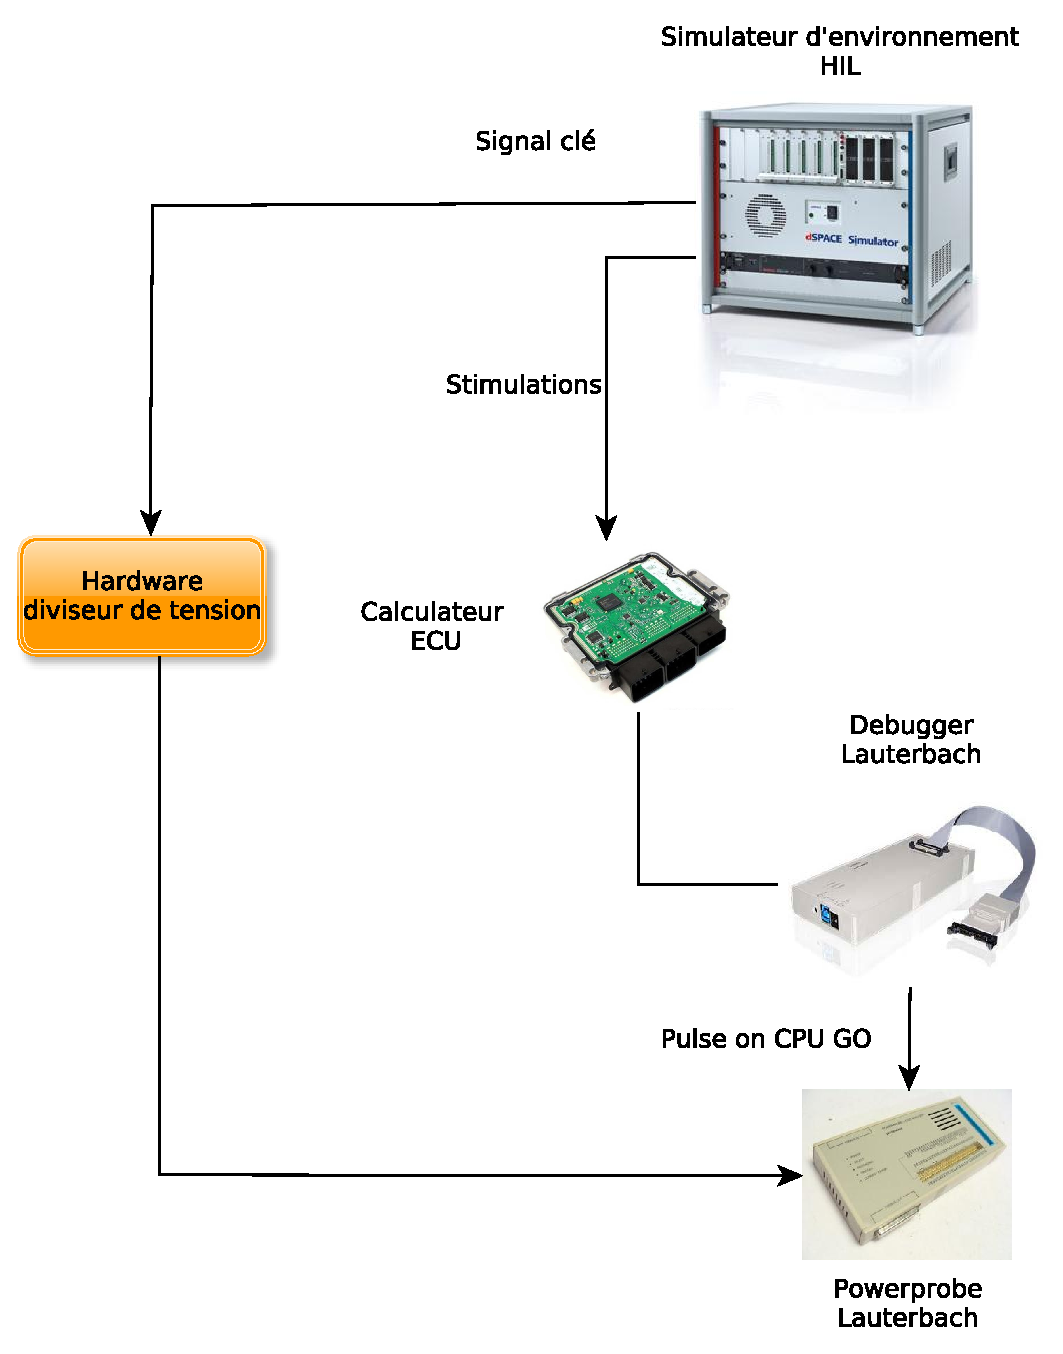
\includegraphics[width=0.42\linewidth]{contents/images/tracesSync}
\caption{Configuration des équipements de la table de tests}
\label{fig:tracesSync}
\end{figure}


Le \textit{PowerProbe} se branche simplement en série sur le \textit{debugger}, un port est prévu à cet effet, il faut ensuite configurer correctement le \textit{debugger} via des commandes spécifiques permettant d'envoyer une pulse au démarrage de l'ECU. 

Le HiL permet de relire les valeurs en sortie du dspace, il est ainsi possible de brancher un fil au niveau de la sortie du signal clé, et de le relier à une entrée du \textit{PowerProbe}. Celui-ci enregistrera à échantillonnage fixe le signal sur l'entrée correspondante. 


\begin{remarque}
Il a été nécessaire d'avoir un petit étage \textit{hardware} entre le HiL et le \textit{PowerProbe}. En effet, le signal clé d'une voiture est en 13 Volts, et peut monter jusqu'à plus de 20 volts pour un camion. Or notre équipement \textit{PowerProbe} ne peut accepter des voltages aussi conséquents, une équipe au sein de Continental nous a fabriqué un équipement permettant de sortir une tension bien plus faible afin d'éviter d'endommager le \textit{PowerProbe}. Cet étage est branché entre le HiL et le \textit{PowerProbe}. 

À terme, il sera nécessaire d'avoir plusieurs de ces adaptateurs hardware afin de les fournir aux différentes équipes de tests, ceux-ci devront pouvoir les brancher facilement.
\end{remarque}
